\subsection{Joists}

\subsubsection{Corridor floor sheathing}
Three layers of 4x8 foot, 19/32 plywood panels are installed as corridor floor sheathing over corridors joists (nominal 3.5 inch wide) spaced 32 inches on center. The panels are installed with the long panel direction (strength axis) perpendicular to the corridor joists. The design loads are:

\begin{align}
  q_{live}&= 1.92\ kN/m^2 (40\ psf) \\
  q_{dead}&= 0.72\ kN/m^2 (15\ psf)
\end{align}

The allowable live load deflection is span/540 and the allowable total load deflection span/360.

\paragraph{Structural design of the panels.}

\subparagraph{Mechanical properties of the plywood panel.}
The mechanical properties used to compute the floor deflection are the elastic modulus $E= 4200\ MPa$ and its thickness $t= 15.09\ mm$ (19/32 inch). Each layer works independently, otherwise said, they are connected only over the joists. 


\subparagraph{Bending stiffness.}
The deflection obtained under live load is:

\begin{equation}
  \Delta_{LL}= 1.34\ mm= \frac{span}{607} < \frac{span}{540} \implies OK
\end{equation}

\noindent and the deflection under total load is:

\begin{equation}
  \Delta_{TL}= 1.84\ mm= \frac{span}{441} < \frac{span}{360} \implies OK
\end{equation}

\subparagraph{Bending strength.}
The allowable bending stress for the 5-ply plywood panel is $F_b= 4.33\ MPa$ (the panel grade and construction factors are already been applied to this capacity). The load duration factor for the live load on the corridor is $C_D= 1.6$. The adjusted allowable bending stress is therefore $F'_b= 6.94\ MPa$.\\

The maximum bending stress obtained under total load (three-span condition) is:

\begin{equation}
  \sigma_{max}= 1.69\ MPa < 6.94\ MPa = F'_b \implies OK
\end{equation}


\subparagraph{Shear strength.}
The allowable shear stress of the panel is $F_v= 0.2\ MPa$ and the adjusted allowable shear stress is (under the same conditions that we used for the bending stress) $F'_v= 0.33\ MPa$.\\

The maximum shear stress obtained under total load is:

\begin{equation}
  \tau_{max}= 0.04\ MPa < 0.33\ MPa = F'_v \implies OK
\end{equation}

\paragraph{Fire design of the panels.}
According the table \ref{tb_fire_resistance_wallboard_membranes} the time assigned to a 19/32 inch panel is 15 minutes, so after 30 minutes of fire only one of the three panels remains in place. Accordingly, we perform the bending and shear checks to the remaining panel.

\subparagraph{Bending strength.}
The maximum bending stress obtained under total load (three-span condition) is:

\begin{equation}
  \sigma_{max}= 4.59\ MPa < 6.94\ MPa = F'_b \implies OK
\end{equation}


\subparagraph{Shear strength.}
The maximum shear stress obtained under total load is:

\begin{equation}
  \tau_{max}= 0.12\ MPa < 0.33\ MPa = F'_v \implies OK
\end{equation}


\begin{table}
  \begin{center}
    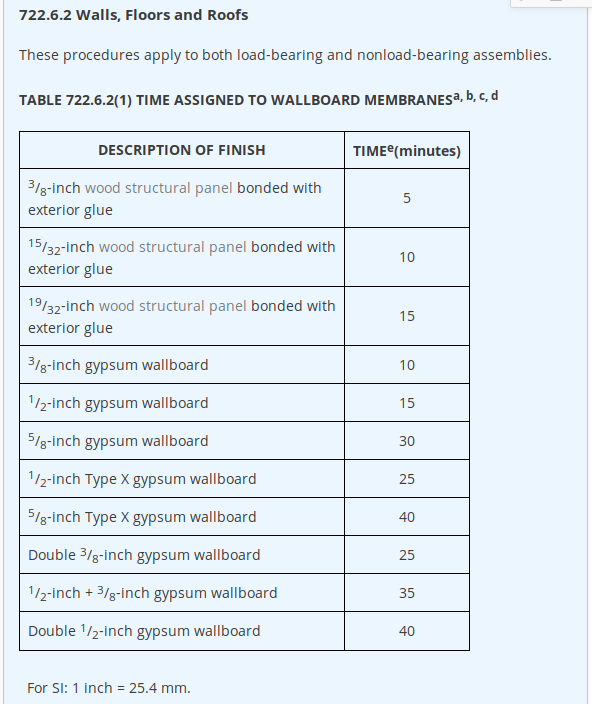
\includegraphics[width= 90mm]{figures/fire_resistance_wallboard_membranes}
  \end{center}
  \caption{Time assigned to wallboard membranes}\label{tb_fire_resistance_wallboard_membranes}
\end{table}


\subsubsection{Corridor Joists}
Simply supported 3.5x6 LVL floor joists span a maximum of $L= 2.49\ m$ (\unit[94.25]{inches}) and are spaced at $s= 0.81\ m$ (\unit[32]{inches}). The design loads are:

\begin{align}
  q_{live}&= 1.92\ kN/m^2 (40\ psf) \\
  q_{dead}&= 0.72\ kN/m^2 (15\ psf)
\end{align}

Timber decking nailed to the compression edge of the joists provides lateral bracing for at least the same fire resistance time as the joists (i.e. $C_L= 1.0$).

\paragraph{Structural design of the joist.}

\subparagraph{Loads.}

\begin{equation}
  w_{load}= s \cdot (q_{dead}+q_{live})= 1.56\ kN/m
\end{equation}

\subparagraph{Internal forces.}

\noindent Maximum induced moment:

\begin{equation}
  M_{max}= w_{load} \frac{L^2}{8}= 1.54\ kN m
\end{equation}

\noindent Maximum induced shear:

\begin{equation}
  V_{max}= w_{load} \frac{L}{2}= 2.57\ kN
\end{equation}

\subparagraph{Joist mechanical properties.}

\noindent Joist section modulus:
\begin{equation}
  S_s= 344.13 \times 10^{-6}\ m^3
\end{equation}

\noindent Tabulated bending stress:
\begin{equation}
  F_b= 21.59\ MPa
\end{equation}


\noindent Adjusted allowable bending stress with $C_r= 1.0$, $C_D= 1.0$,$C_M= 1.0$, $C_t= 1.0$,$C_V= 0.62$:
\begin{equation}
  F'_b= 13.59\ MPa
\end{equation}

\noindent Tabulated shear stress:
\begin{equation}
  F_v= 1.97\ MPa
\end{equation}

\noindent Adjusted allowable shear stress with $C_D= 1.0$,$C_M= 1.0$, $C_t= 1.0$:
\begin{equation}
  F'_v= 1.97\ MPa
\end{equation}

\subparagraph{Structural bending check.}

\noindent Design resisting moment:

\begin{equation}
  M'_s= 4.67\ kN m
\end{equation}

\noindent Structural bending check: $M'_s = 4.67 > 1.54 = M_{max} \implies OK$

\subparagraph{Structural shear check.}

\noindent Design resisting shear:
\begin{equation}
  V'_s= 17.74\ kN
\end{equation}

\noindent Structural shear check: $V'_s = 17.74 > 2.57 = V_{max} \implies OK$

\paragraph{Fire design of the joist.}
For the fire design of the joist, mass loss due to charring is conservatively neglected, so the loading is unchanged. Therefore, the maximum induced moment and shear are unchanged. The fire resistance must be calculated.

\subparagraph{Mechanical properties of the burned section.}

\noindent Effective char depth:
\begin{equation}
  a_{eff}= 0.7 \times 10^{-3} \times 30 + 7 \times 10^{-3}= 28\ mm
\end{equation}

\noindent section modulus for a joist exposed on three sides:
\begin{equation}
  S_s= 84.86 \times 10^{-6}\ m^3
\end{equation}

\noindent shear area for a beam exposed on three sides:
\begin{equation}
  A_f= 40.93\ cm^2
\end{equation}

\noindent Adjusted allowable bending stress with $C_{fire}= 2.85$, $C_r= 1.0$, $C_D= 1.0$,$C_M= 1.0$, $C_t= 1.0$,$C_V= 0.62$:
\begin{equation}
  F'_{b,f}= 38.74\ MPa
\end{equation}

\noindent Adjusted allowable shear stress with  $C_{fire}= 2.85$, $C_D= 1.0$,$C_M= 1.0$, $C_t= 1.0$:
\begin{equation}
  F'_{v,f}= 5.40\ MPa
\end{equation}

\subparagraph{Structural bending check.}

\noindent Design resisting moment:

\begin{equation}
  M'_f= 3.28\ kN m
\end{equation}

\noindent Structural bending check: $M'_s = 3.28 > 1.54 = M_{max} \implies OK$

\subparagraph{Structural shear check.}

\noindent Design resisting shear:
\begin{equation}
  V'_f= 14.74\ kN
\end{equation}

\noindent Structural shear check: $V'_s = 14.74 > 2.57 = V_{max} \implies OK$

\subsubsection{Joists under storage/HVAC floor}
Simply supported 3.5x9.25 LVL floor joists span a maximum of $L= 2.9\ m$ and are spaced at $s= 0.81\ m$ (\unit[32]{inches}). The design loads are:

\begin{align}
  q_{live}&= 5.99\ kN/m^2 (125\ psf) \\
  q_{dead}&= 0.72\ kN/m^2 (15\ psf)
\end{align}

Timber decking nailed to the compression edge of the joists provides lateral bracing (i.e. $C_L= 1.0$).

\paragraph{Structural design of the joist.}

\subparagraph{Loads.}

\begin{equation}
  w_{load}= s \cdot (q_{dead}+q_{live})= 5.45\ kN/m
\end{equation}

\subparagraph{Internal forces.}

\noindent Maximum induced moment:

\begin{equation}
  M_{max}= w_{load} \frac{L^2}{8}= 5.79\ kN m
\end{equation}

\noindent Maximum induced shear:

\begin{equation}
  V_{max}= w_{load} \frac{L}{2}= 7.94\ kN
\end{equation}

\subparagraph{Joist mechanical properties.}

\noindent Joist section modulus:
\begin{equation}
  S_s= 817.90 \times 10^{-6}\ m^3
\end{equation}

\noindent Tabulated bending stress:
\begin{equation}
  F_b= 20.58\ MPa
\end{equation}


\noindent Adjusted allowable bending stress with $C_r= 1.0$, $C_D= 1.0$,$C_M= 1.0$, $C_t= 1.0$
\begin{equation}
  F'_b= 20.58\ MPa
\end{equation}

\noindent Tabulated shear stress:
\begin{equation}
  F_v= 1.97\ MPa
\end{equation}

\noindent Adjusted allowable shear stress with $C_D= 1.0$,$C_M= 1.0$, $C_t= 1.0$:
\begin{equation}
  F'_v= 1.97\ MPa
\end{equation}

\subparagraph{Structural bending check.}

\noindent Design resisting moment:

\begin{equation}
  M'_s= 16.83\ kN m
\end{equation}

\noindent Structural bending check: $M'_s = 16.83 > 5.79 = M_{max} \implies OK$

\subparagraph{Structural shear check.}

\noindent Design resisting shear:
\begin{equation}
  V'_s= 27.36\ kN
\end{equation}

\noindent Structural shear check: $V'_s = 27.36 > 7.94 = V_{max} \implies OK$

\subparagraph{Bending stiffness.}
The deflection obtained under live load is:

\begin{equation}
  \Delta_{LL}= 3.45\ mm= \frac{span}{845} < \frac{span}{540} \implies OK
\end{equation}

\noindent and the deflection under total load is:

\begin{equation}
  \Delta_{TL}= 3.86\ mm= \frac{span}{754} < \frac{span}{360} \implies OK
\end{equation}

